\section{Implementation of Classical IPC Mechanisms}
\label{sec:ipc_implementation}

This section details the low-level implementation mechanics, system calls, synchronization protocols, memory layouts, and error-handling strategies of the six classical Linux IPC mechanisms implemented in Mini-A-IPC. Table~\ref{tab:ipc_comparison} provides an architectural comparison of all six mechanisms, and Fig.~\ref{fig:ipc_mechanisms} illustrates their communication topologies.

\begin{table*}[t]
\centering
\caption{Architectural Comparison of Evaluated Linux Inter-Process Communication Mechanisms}
\label{tab:ipc_comparison}
\scriptsize
\begin{tabular}{lp{2.4cm}ccccp{3.2cm}p{3.2cm}}
\toprule
\textbf{Mechanism} & \textbf{Data Structure / Model} & \textbf{Data Copies} & \textbf{Buffering Space} & \textbf{Boundary Semantics} & \textbf{Max Payload Limit} & \textbf{Synchronization Primitive} & \textbf{Key System Calls} \\
\midrule
\textbf{Anonymous Pipe} & Kernel page ring buffer & 2 & Kernel & Byte-stream & Bounded by pipe buffer (64 KB) & Implicit (kernel blocking queue) & \texttt{pipe2}, \texttt{read}, \texttt{write}, \texttt{close} \\
\textbf{Named FIFO} & Filesystem inode pipe & 2 & Kernel & Byte-stream & Bounded by pipe buffer (64 KB) & Implicit (kernel blocking queue) & \texttt{mkfifo}, \texttt{open}, \texttt{read}, \texttt{write} \\
\textbf{System V MQ} & Kernel linked message list & 2 & Kernel & Message-oriented & \texttt{MSGMAX} / \texttt{MSGMNB} sysctl & Implicit (message type filtering) & \texttt{msgget}, \texttt{msgsnd}, \texttt{msgrcv}, \texttt{msgctl} \\
\textbf{POSIX MQ} & Virtual \texttt{/dev/mqueue} file & 2 & Kernel & Priority message & Dynamic \texttt{mq\_msgsize} (max 10 msgs) & Implicit (priority queue lock) & \texttt{mq\_open}, \texttt{mq\_send}, \texttt{mq\_receive} \\
\textbf{POSIX SHM} & Memory-mapped pages & \textbf{0} & Userspace & Structured mailbox & 1,024 B (\texttt{SHM\_MAX\_PAYLOAD}) & Explicit (POSIX unnamed semaphores) & \texttt{shm\_open}, \texttt{mmap}, \texttt{sem\_wait}, \texttt{sem\_post} \\
\textbf{Unix Domain Skt} & Socket buffer (\texttt{sk\_buff}) & 2 & Kernel & Byte-stream & Socket buffer auto-tuning & Implicit (BSD socket transport) & \texttt{socket}, \texttt{bind}, \texttt{connect}, \texttt{send}, \texttt{recv} \\
\textbf{Kernel Mailbox} & Custom char device & 2 & Kernel & Bounded byte-stream & 64 KB ring capacity & Sleepable mutex + wait queues & \texttt{open}, \texttt{read}, \texttt{write}, \texttt{poll}, \texttt{release} \\
\bottomrule
\end{tabular}
\end{table*}


\begin{figure*}[t]
\centering
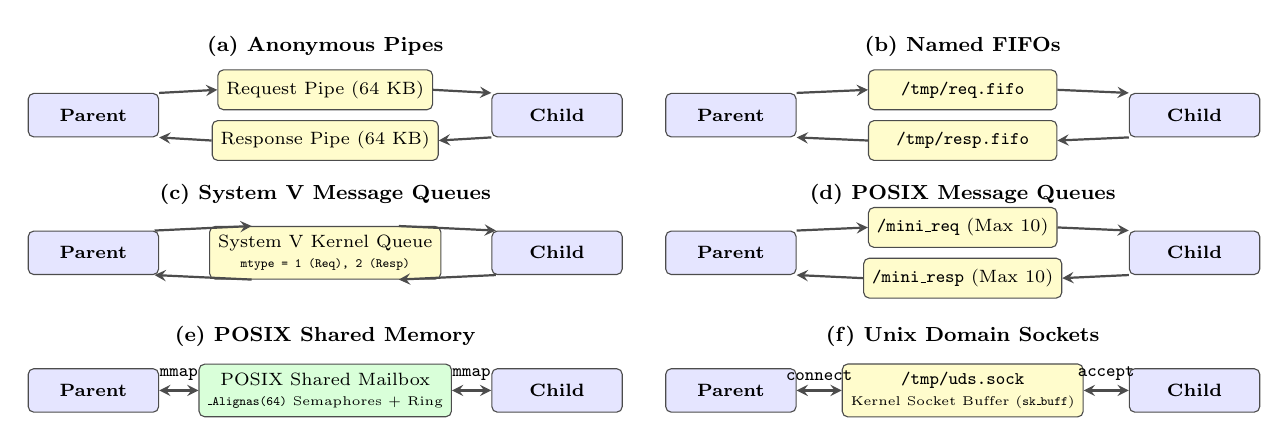
\begin{tikzpicture}[
    scale=0.92, every node/.style={transform shape},
    proc/.style={draw=black!70, fill=blue!10, rounded corners=2pt, font=\scriptsize\bfseries, minimum width=1.8cm, minimum height=0.6cm, align=center},
    buffer/.style={draw=black!70, fill=yellow!20, rounded corners=2pt, font=\scriptsize, minimum width=2.6cm, minimum height=0.55cm, align=center},
    shmbuf/.style={draw=black!70, fill=green!15, rounded corners=2pt, font=\scriptsize, minimum width=3.0cm, minimum height=0.55cm, align=center},
    arr/.style={->, >=stealth, thick, draw=black!70},
    darr/.style={<->, >=stealth, thick, draw=black!70}
]

% Row 1: Anonymous Pipes & Named FIFOs
\node[proc] (p1) at (0, 3.8) {Parent};
\node[buffer] (b1) at (3.2, 4.15) {Request Pipe (64 KB)};
\node[buffer] (b2) at (3.2, 3.45) {Response Pipe (64 KB)};
\node[proc] (c1) at (6.4, 3.8) {Child};
\draw[arr] (p1.north east) -- (b1.west);
\draw[arr] (b1.east) -- (c1.north west);
\draw[arr] (c1.south west) -- (b2.east);
\draw[arr] (b2.west) -- (p1.south east);
\node[font=\footnotesize\bfseries] at (3.2, 4.75) {(a) Anonymous Pipes};

\node[proc] (p2) at (8.8, 3.8) {Parent};
\node[buffer] (f1) at (12.0, 4.15) {\texttt{/tmp/req.fifo}};
\node[buffer] (f2) at (12.0, 3.45) {\texttt{/tmp/resp.fifo}};
\node[proc] (c2) at (15.2, 3.8) {Child};
\draw[arr] (p2.north east) -- (f1.west);
\draw[arr] (f1.east) -- (c2.north west);
\draw[arr] (c2.south west) -- (f2.east);
\draw[arr] (f2.west) -- (p2.south east);
\node[font=\footnotesize\bfseries] at (12.0, 4.75) {(b) Named FIFOs};

% Row 2: System V MQ & POSIX MQ
\node[proc] (p3) at (0, 1.9) {Parent};
\node[buffer] (mq1) at (3.2, 1.9) {System V Kernel Queue\\ \tiny \texttt{mtype = 1 (Req), 2 (Resp)}};
\node[proc] (c3) at (6.4, 1.9) {Child};
\draw[arr] (p3.20) -- (mq1.160);
\draw[arr] (mq1.20) -- (c3.160);
\draw[arr] (c3.200) -- (mq1.340);
\draw[arr] (mq1.200) -- (p3.340);
\node[font=\footnotesize\bfseries] at (3.2, 2.7) {(c) System V Message Queues};

\node[proc] (p4) at (8.8, 1.9) {Parent};
\node[buffer] (pmq1) at (12.0, 2.25) {\texttt{/mini\_req} (Max 10)};
\node[buffer] (pmq2) at (12.0, 1.55) {\texttt{/mini\_resp} (Max 10)};
\node[proc] (c4) at (15.2, 1.9) {Child};
\draw[arr] (p4.north east) -- (pmq1.west);
\draw[arr] (pmq1.east) -- (c4.north west);
\draw[arr] (c4.south west) -- (pmq2.east);
\draw[arr] (pmq2.west) -- (p4.south east);
\node[font=\footnotesize\bfseries] at (12.0, 2.7) {(d) POSIX Message Queues};

% Row 3: POSIX SHM & Unix Domain Sockets
\node[proc] (p5) at (0, 0.0) {Parent};
\node[shmbuf] (shm) at (3.2, 0.0) {POSIX Shared Mailbox\\ \tiny \texttt{\_Alignas(64)} Semaphores + Ring};
\node[proc] (c5) at (6.4, 0.0) {Child};
\draw[darr] (p5) -- node[above, font=\scriptsize] {\texttt{mmap}} (shm);
\draw[darr] (shm) -- node[above, font=\scriptsize] {\texttt{mmap}} (c5);
\node[font=\footnotesize\bfseries] at (3.2, 0.75) {(e) POSIX Shared Memory};

\node[proc] (p6) at (8.8, 0.0) {Parent};
\node[buffer] (uds) at (12.0, 0.0) {\texttt{/tmp/uds.sock}\\ \tiny Kernel Socket Buffer (\texttt{sk\_buff})};
\node[proc] (c6) at (15.2, 0.0) {Child};
\draw[darr] (p6) -- node[above, font=\scriptsize] {\texttt{connect}} (uds);
\draw[darr] (uds) -- node[above, font=\scriptsize] {\texttt{accept}} (c6);
\node[font=\footnotesize\bfseries] at (12.0, 0.75) {(f) Unix Domain Sockets};

\end{tikzpicture}

\caption{Communication topologies and data flows of the six classical Linux Inter-Process Communication mechanisms implemented in Mini-A-IPC: (a) Anonymous Pipes, (b) Named FIFOs, (c) System V Message Queues, (d) POSIX Message Queues, (e) POSIX Shared Memory, and (f) Unix Domain Sockets.}
\label{fig:ipc_mechanisms}
\end{figure*}

\subsection{Anonymous Pipes (\texttt{src/ipc\_pipe.c})}
Anonymous pipes provide unidirectional byte-stream channels managed by the Linux VFS. Full-duplex round-trip exchange requires two distinct pipe pairs: \texttt{request\_pipe[2]} and \texttt{response\_pipe[2]}.
Following \texttt{pipe()} invocation, \texttt{fork()} clones the parent process. The child immediately closes the write end of the request pipe (\texttt{request\_pipe[1]}) and the read end of the response pipe (\texttt{response\_pipe[0]}). Conversely, the parent closes \texttt{request\_pipe[0]} and \texttt{response\_pipe[1]}. Explicitly closing unused descriptors ensures proper EOF propagation when a peer terminates.
Because pipes do not preserve message boundaries, we implement robust \texttt{read\_all()} and \texttt{write\_all()} transfer loops that handle partial transfers, check for \texttt{EINTR} interruptions, and detect unexpected EOF. To prevent abnormal termination when writing to a broken pipe, the implementation configures \texttt{sigaction} to set \texttt{SIGPIPE} to \texttt{SIG\_IGN}, ensuring \texttt{write()} returns $-1$ with \texttt{errno = EPIPE}.

\subsection{Named Pipes (\texttt{src/ipc\_fifo.c})}
Named pipes (FIFOs) extend pipe functionality across unrelated processes via the filesystem namespace.
Private FIFO nodes are instantiated in \texttt{/tmp} with PID-isolated paths: \texttt{/tmp/mini\_aipc\_req\_<pid>.fifo} and \texttt{/tmp/mini\_aipc\_resp\_<pid>.fifo}. Nodes are created using \texttt{mkfifo()} with restrictive \texttt{0600} permissions (read/write by owner only), mitigating local unauthorized access vulnerabilities.
Opening a FIFO blocks until both read and write endpoints are open. To prevent mutual deadlock between parent and child, the implementation enforces an asymmetric open sequence: the child opens the request FIFO for reading (\texttt{O\_RDONLY}) and subsequently opens the response FIFO for writing (\texttt{O\_WRONLY}). The parent reverses this order, opening the request FIFO for writing (\texttt{O\_WRONLY}) and then the response FIFO for reading (\texttt{O\_RDONLY}). Both FIFOs are explicitly unlinked via \texttt{unlink()} upon benchmark completion or error bailout.

\subsection{System V Message Queues (\texttt{src/ipc\_sysv\_mq.c})}
System V IPC operates within a kernel-maintained global message space.
Mini-A-IPC allocates a private queue using \texttt{msgget(IPC\_PRIVATE, IPC\_CREAT | IPC\_EXCL | 0600)}. Specifying \texttt{IPC\_PRIVATE} guarantees the allocation of a unique, unshared queue descriptor (\texttt{msqid}).
Rather than allocating multiple queues, full-duplex communication is multiplexed over a single queue using message types: parent sends requests with \texttt{mtype = 1L} (\texttt{MSG\_TYPE\_REQ}); child blocks on \texttt{msgrcv()} for type \texttt{1L} and responds with \texttt{mtype = 2L} (\texttt{MSG\_TYPE\_RESP}); parent blocks on \texttt{msgrcv()} for type \texttt{2L}.
A \texttt{SIGCHLD} signal handler is installed with \texttt{sa\_flags = 0} (explicitly omitting \texttt{SA\_RESTART}). If the child dies, the blocking \texttt{msgrcv()} call in the parent immediately unblocks with \texttt{EINTR}, allowing the parent to reap the child and teardown the queue via \texttt{msgctl(msqid, IPC\_RMID, NULL)}.

\subsection{POSIX Message Queues (\texttt{src/ipc\_posix\_mq.c})}
POSIX message queues provide structured priority messaging through the virtual \texttt{/dev/mqueue} filesystem.
Queues are allocated via \texttt{mq\_open()} with names formatted as \texttt{/mini\_aipc\_req\_<pid>} and \texttt{/mini\_aipc\_resp\_<pid>}. The queue attribute structure (\texttt{struct mq\_attr}) explicitly configures \texttt{mq\_maxmsg = 10} and \texttt{mq\_msgsize = payload\_size}. The value \texttt{mq\_maxmsg = 10} strictly respects the unprivileged Linux kernel default ceiling (\texttt{/proc/sys/fs/mqueue/msg\_max}). Dynamically sizing \texttt{mq\_msgsize} to the exact payload size avoids kernel allocation rejection while fulfilling POSIX buffer requirements. Descriptors are closed via \texttt{mq\_close()} and names unlinked via \texttt{mq\_unlink()}.

\subsection{POSIX Shared Memory (\texttt{src/ipc\_shm.c})}
POSIX shared memory provides direct memory access without intermediate kernel buffering.
False sharing across CPU cores severely degrades multicore shared memory performance. In Mini-A-IPC, the shared mailbox structure \texttt{shared\_mailbox\_t} enforces strict cache-line alignment (\texttt{\_Alignas(64)}) across all fields: semaphores \texttt{request\_empty}/\texttt{full} reside in cache line 0, response semaphores in line 1, producer payload buffer in line 2+, and consumer payload buffer in line $N$+. By isolating producer-written fields from consumer-written fields across separate 64-byte cache lines, cross-core L1/L2 cache invalidations during lockstep exchanges are eliminated.
The shared mailbox enforces a bounded payload limit of $\le 1,024$~bytes (\texttt{SHM\_MAX\_PAYLOAD}). Payloads $> 1024$~bytes are rejected with \texttt{errno = EMSGSIZE}, providing deterministic zero-allocation execution.
To eliminate timer polling overhead, the hot loop employs fast \texttt{sem\_wait()}, paired with a non-restarting \texttt{SIGCHLD} handler that breaks \texttt{sem\_wait()} with \texttt{EINTR} in $< 1\,\mu\text{s}$ upon child termination.

\subsection{Unix Domain Sockets (\texttt{src/ipc\_uds.c})}
Unix domain sockets provide bidirectional stream communication through the local networking subsystem.
The parent process instantiates a stream socket endpoint (\texttt{socket(AF\_UNIX, SOCK\_STREAM, 0)}), binds to \texttt{/tmp/mini\_aipc\_uds\_<pid>.sock}, and issues \texttt{listen(listen\_fd, 1)} \textit{prior} to invoking \texttt{fork()}. This ensures the server endpoint is active and listening before the client connects, eliminating connection refusal races.
The child calls \texttt{accept()} to obtain a dedicated connection descriptor (\texttt{conn\_fd}), while the parent creates a client socket and executes \texttt{connect()}. Transfers are managed using robust \texttt{send\_all()} and \texttt{recv\_all()} byte-streaming loops.
